\subsubsection{Rucksack-Problem (Greedy-Algorithmus)}
Nun betrachten wir unsere Problemstellung als ein Rucksack-Problem (Knapsack-Problem). Das Volumen des Rucksacks entspricht unserem Kostenbudget. Unser Ziel ist es nun, diesen Rucksack m"oglichst sinnvoll und mit dem f"ur uns besten Nutzen zu packen. In unserem Fall entspricht dies einem m"oglichst kleinen Fehler. Wir haben zum Packen unseres Rucksacks unterschiedliche G"uter mit entsprechendem Gewicht zur Verf"ugung. Bei uns sind diese G"uter die Samples auf den unterschiedlichen Level mit den Kosten $2^l$.
Eine M"oglichkeit solche Probleme zu l"osen sind Greedy-Algorithmen.
Zuerst gilt zu kl"aren, was unter einem Greedy-Algorithmus zu verstehen ist. Hierbei orientiere ich mich an \cite{Greedy}.\\
Greedy-Algorithmen bilden eine spezielle Klasse von Optimierungsalgorithmen. Sie zeichnen sich dadurch aus, dass sie schrittweise den Folgezustand ausw"ahlen, der zum Zeitpunkt der Wahl den gr"o"sten Gewinn bzw. das beste Ergebnis (berechnet durch eine Bewertungsfunktion) verspricht. Greedy-Algorithmen sind oft schnell, l"osen viele Probleme aber nicht optimal.\\[0,1cm]

Ein gieriger Algorithmus m"ochte in jedem Teilschritt so viel wie m"oglich im Hinblick auf die Vorgabe erreichen. Eine Anwendung eines solchen Greedy-Algorithmus im t"aglichen Leben ist beispielsweise die Herausgabe von Wechselgeld.\\[0,1cm]

Das Ziel ist es, eine bestimmte Geldsumme in m"oglichst wenigen Schritten herauszugeben.
Vorgehen nach Greedy: Man nimmt die gr"o"ste M"unze unter dem Zielwert und zieht sie von diesem ab. Man macht dies solange, bis der Zielwert gleich Null ist. Will man beispielsweise 79 Cent zur"uckgeben, f"angt der Algorithmus sofort mit dem h"ochsten M"unzwert an und macht weiter, bis er den niedrigsten M"unzwert erreicht hat (falls das n"otig ist): 
\begin{align*}
79=50 + 20 + 5 + 2 +2
\end{align*}
In diesem Fall klappt das perfekt. Greedy-Algorithmen berechnen jeweils ein  \glqq lokales Optimum\grqq{ } in jedem Schritt und k"onnen daher eventuell ein \glqq globales Optimum\grqq{ } verpassen.\\ Hierf"ur ein Beispiel:\\
Der Zielwert sei $15$. Es stehen M"unzen mit den Werten 1, 5 und 11 zur Verf"ugung.\\
Die optimale L"osung ist $15=5+5+5$. Greedy liefert uns jedoch $15=11+1+1+1+1$.\\[0,5cm]
Mein Ziel ist es nun, durch solch eine Vorgehenswei"se meine optimalen Sampleanzahlen zu bestimmen. In unserem Fall sind wir \glqq gierig\grqq{ } auf Level $1$, da diese Samples, wie schon beschrieben, den gr"o"sten Faktor in der Fehlerfunktion haben.\\
Haben wir zum Beispiel ein Kostenbudget von $C=100$ gegeben, w"urde uns Greedy $50$ Samples auf Level 1 mit Kosten 2 liefern.
Gebe ich vor $2$ Level zu wollen, w"are das Ergebnis $100=48 \cdot 2+ 1\cdot 4$. Dass dieses Ergebnis nicht optimal, ist klar.\\
Mein Ziel ist es nun, durch Umverteilen der Samples das Optimum zu finden.
Dies bedeutet, ich gebe wie auch bei der Lagrange-Methode zuerst eine feste Levelanzahl vor. Der Ausgangspunkt nach Greedy wird immer sein, so viele Samples auf Level 1 wie m"oglich zu nehmen und auf den anderen jeweils nur einen. Solange sich das Ergebnis dadurch verbessert und die Sample Anzahl nicht 0 oder negativ wird, verteile ich Samples von Level 1 auf Level 2. Wird das Ergebnis schlechter, beginne ich mit dem Umverteilen von Level 2 auf Level 3 usw. \\
Da sich die Kosten zweier aufeinanderfolgender Level um den Faktor 2 unterscheiden, folgt, dass die Erh"ohung um ein Sample auf Level $l$ eine Verringerung der Sampleanzahl um zwei bei Level $l-1$ ben"otigt.
Au"serdem brechen wir ab bzw. geben eine Warnung aus, falls wir auf mehreren Leveln hintereinander nur 1 Sample nehmen w"urden. Dies passiert, falls wir nicht mehr weiter umverteilen k"onnen. Da unsere Samples eine monoton fallende Folge bilden m"ussen, macht solch eine Verteilung keinen Sinn. \newpage
Ein Beispiel: Kostenbudget von $C=100$ und eine gew"unschte Levelanzahl von $5$. \\
Das Ergebnis ist:\\
\begin{center}
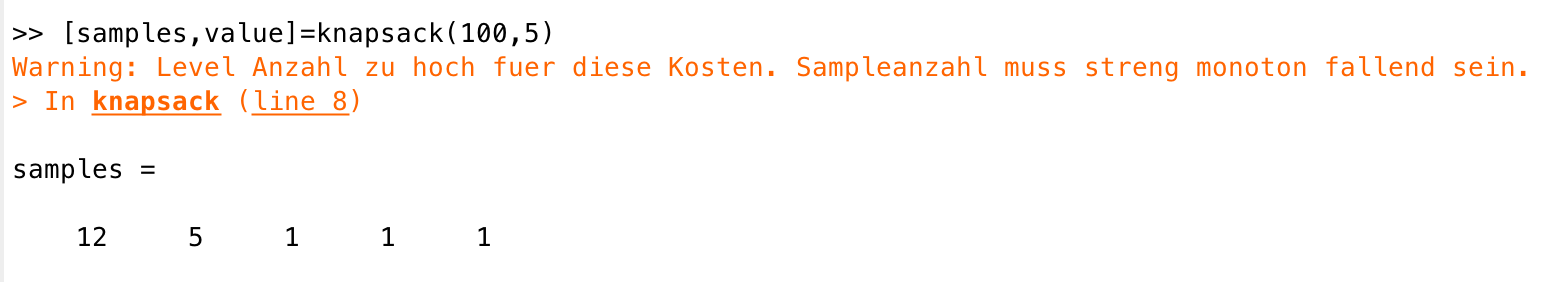
\includegraphics[width=15cm]{Knapsack5.png}
\end{center}
Es konnte also von Level 2 auf Level 3 nicht mehr umverteilt werden, ohne das Ergebnis zu verschlechtern. Deshalb bleiben dann auch alle anderen Samplezahlen unver"andert. Bei einem Kostenbudgets von $100$ ist es also nicht mehr sinnvoll $5$ Level zu fordern. Im Vergleich hierzu das Ergebnis bei nur $4$ Leveln:\\
\begin{center}
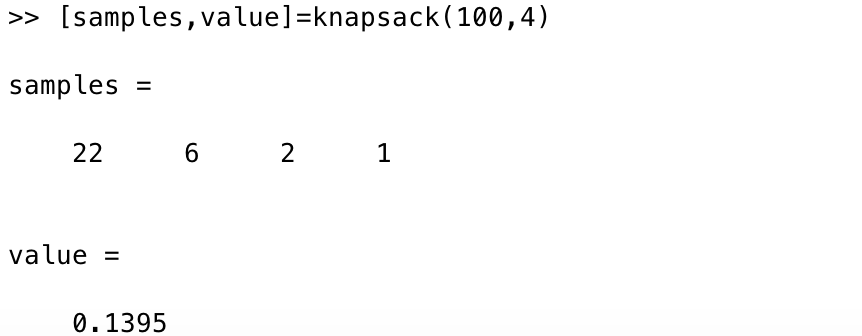
\includegraphics[width=10cm]{Knapsack4.png}
\end{center}
Um nachfolgenden Algorithmus besser zu verstehen, noch ein paar Vor"uberlegungen:\\
Unsere Ausgangssituation ist es, auf jedem Level ab 2 bis L nur ein Sample zu nehmen und so viele wie m"oglich auf Level 1. Hier muss nat"urlich erst "uberpr"uft werden, ob dies "uberhaupt m"oglich ist. Das Kostenbudget k"onnte f"ur die gew"unsche Levelanzahl zu niedrig sein. Ist dies jedoch m"oglich, k"onnen die Kosten der Samples auf Level 2 bis L durch eine geometrische Summe beschrieben werden. N"amlich $\sum_{l=2}^L 1\cdot 2^l = -(1-2^{L+1})-3$. D.h die Sampleanzahl auf Level 1 ist die abgerundete und halbierte (da die Kosten auf Level 1 zwei betragen) Differenz aus dem Kostenbudget und dem Wert der geometrischen Summe.
Auf der n"achsten Seite ist der Algorithmus beschrieben. L ist hierbei die Levelanzahl und cost das vorgegebene Kostenbudget.\\

\begin{algorithm}[H]
\textbf{Knapsack}(cost,L)=\\
samples=(1,...,1) mit L"ange L\\
\eIf{geosum- cost$\geq 2$}{
samples(1)=$\lfloor\frac{(\text{cost-geosum})}{2}\rfloor$\\
value= Fehler, den man mit den samples erh"alt.
}
{Fehler: Levelanzahl f"ur gegebenes Kostenbudget zu hoch!}

\For{l=2 \textbf{to} L}{ 
    \If {samples(l-1)$\leq 2$}{
    \If{(samples(l)=1 und samples(l-1)=1) oder l<L}
    {Breche ab. Levelanzahl zu hoch, da keine monton fallende Folge.}}
 }
\While{1}{
tempsamples=samples\\
tempsamples(l-1)=tempsamples(l-1)-2\\
tempsamples(l)=tempsamples(l)+1\\
tempvalue= Fehler unter tempsamples\\
\eIf{tempvalue >value}{
Abbruch, da Ergebnis schlechter wird.
}
{value=tempvalue\\
samples=tempsamples}
}

\caption{Algorithmus f"ur optimale Sampleanzahl mit der Umverteil-Methode}
\end{algorithm}\vspace{0,3cm}
Um die optimale Levelanzahl zu bestimmen gehen wir analog zu Lagrange vor. Das hei"st wir durchlaufen die einzelnen Level und w"ahlen das mit dem kleinsten $\varepsilon$.\\
Nachfolgend eine Tabelle mit den Ergebnissen:\\
\begin{center}
\begin{tabular}{|c|c|c|}
Kostenbudgets & opt. Levelanzahl & Fehler $\varepsilon$ \\
 \hline
10 & 1 & 0.3261 \\
\hline
100& 4 & 0.1395 \\
\hline
1000& 5 &  0.0562 \\
\hline
10 000& 7 & 0.0206 \\
\hline
100 000& 8 & 0.0082 \\
\hline
1 000 000& 10 &   0.0029 \\
\hline
5 000 000& 11 & 0.0015
 \\
\end{tabular}
\end{center}
Auch hier ist wie bei Lagrange deutlich zu erkennen, dass ein h"oheres Kostenbudget  eine Verbesserung des Fehlers mit sich bringt. 
Die zugeh"origen Sampleverteilungen zur Tabelle sind:
\begin{center}
\begin{tabular}{|c|c|}
Kostenbudgets & Sampleverteilung \\
 \hline
10 & n=5 \\
\hline
100& n=(22, 6 ,2 ,1) \\
\hline
1000& n=(276,58,13,5,1) \\
\hline
10 000& n=(2856,592,124,26,6,3,1) \\
\hline
100 000& n=(29142,6037,1252,260,56,13,4,1) \\
\hline
1 000 000&  n=(292296,60538,12539,2597,539,113,24,7,2,1) \\
\hline
5 000 000& n=(1463266, 303055,62766,13001,2694,558,118 ,25,7,2,1)
 \\
\end{tabular}
\end{center}\vspace{0,3cm}
Wir vergleichen auch diese Methode mit der aus Kapitel 5.1. Wir hatten schon bei Lagrange erw"ahnt, dass Kapitel 5.1 f"ur einen Fehler von $10^{-1}$ 2 Level mit 2629 Samples auf Level 1 und 930 Samples auf Level 2 lieferte. Die Kosten waren 8974.
Unsere Umverteil-Methode liefert f"ur dieses Kostenbudget zwei Level  mit 2629 und 929 Samples. Das bedeutet, dass es hier wie auch schon bei Lagrange  keinen wirklichen Unterschied gibt. Geben wir die Kosten sowie die Levelanzahl vor, erhalten wir wie zu erwarten die selben Ergebnisse wie in Kapitel 5.1. Lassen wir die Levelanzahl jedoch variabel, erhalten wir als Optimum bei diesen Kosten sieben Level und einen Fehler von $0.0215$. 
